\section{MSL Constructs}

There are are a number of stream-oriented languages drawing from
domains such as functional, dataflow, CSP and synchronous
programming~\cite{survey97}. The MSL assumes an
architecture-independent programming language for high-performance
stream programming. It requires that the stream program presented for
execution simply consist of a dataflow graph expressing the
computation. Nodes in the graphs embody computation (e.g., actors,
filters, kernels, some encapsulated code block), and edges imply data
dependencies between input and output buffers attached to the compute
nodes. An example stream graph for an MPEG-2 decoder is shown in
Figure~\ref{fig:mpeg}. Nodes in sequence expose pipeline parallelism,
and nodes in parallel expose task (two branches of a split-join
contain different computation) and data parallelism (branches of a
split-join contain the same computation but on different data).

\begin{figure}[tb]
\begin{center}
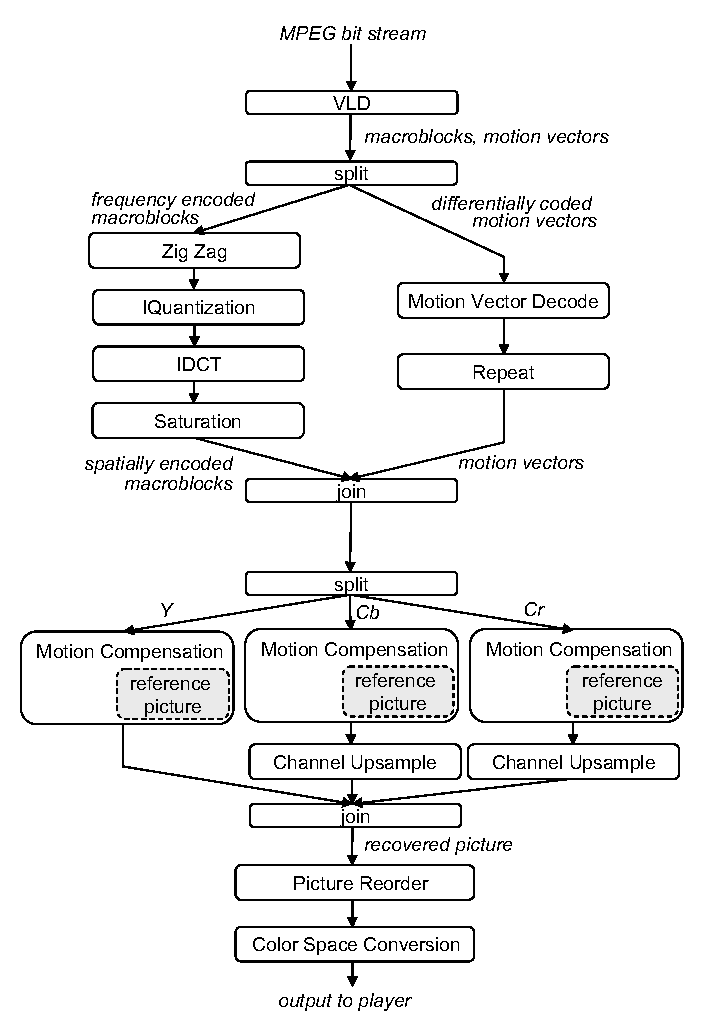
\includegraphics[scale=.55]{figs/mpeg2d}
\end{center}
\caption[MPEG-2 stream graph.]{MPEG-2 stream graph.}
\label{fig:mpeg}
\end{figure}

An execution of a stream program is an ordered sequence of node
firings. Each node follows a set of execution steps that consume a
number of items from each input channel and produce a number of items
onto each output channel.

There are two basic constructs in the MSL: \emph{filters} and
\emph{buffers}. A filter represents a generic actor that exposes a
work function which conceptually runs infinitely. Filters may be
stateful and can read from multiple input buffers and write to multiple
output buffers. While a filter can correspond directly to a
single filter in the program, a compiler can also perform
optimizations such as fusing multiple filters into a single
coarse grained MSL filter~\cite{asplos02}. Work functions are opaque to the MSL.

\emph{Buffers} are contiguous regions of data that are reserved for
temporarily storing input or output data. All buffers are circular,
and the MSL library maintains head and tail pointers for each buffer
that indicate where data begins and ends. Conceptually, a buffer has
front and back ends; data toward the front of a buffer originated
earlier in the execution of the program.

Conceptually, a filter consists of two major components, \emph{code}
and \emph{state}, as well as basic properties that describe its work
function such as the number of input and output buffers. \emph{Code}
is a single contiguous block of arbitrary data that may contain
constant data and instructions that define multiple functions; the MSL
only requires that it contain a function with a specific signature
that is used as the work function. Code for a filter is intended to be
a single modular component that can be easily relocated to different
cores. On a distributed memory architecture where each core has a
dedicated local store (LS), code should not reference absolute
addresses (e.g., absolute branches or loads) or modify
itself\footnote{These restrictions may be ignored if it is acceptable
to not relocate filter code, or to pin the code to a single core.}.

Furthermore, code should not contain any references to mutable global
variables. Instead, code should declare and access mutable state
through fields that are local to a filter. \emph{State} contains all
mutable data that must be maintained across iterations of the work
function. Hence, state for different filters is disjoint, and filters
do not share data.

Before a filter can run on a core, it must be loaded onto the core
through the MSL library. Although the filter code and state must
reside on a core's LS while the filter work function is running, every
filter must have a permanent store location in memory. The MSL
provides facilities for loading code onto cores and copying state
between local store and memory. Note that although we refer to a
core's local store, the MSL concepts and constructs are applicable on
shared memory multicores. The locality restrictions are generally
advantageous for cache-based architectures, NUMA architectures, and
distributed memory architectures.

A user (e.g., compiler or scheduler) provides the library with the
properties of the filter and the local store address of its work
function; the library initializes a control block that describes the
loaded filter in local store. The LS address of the control block
identifies the loaded filter in all future operations until it is
unloaded. If the filter is stateful, the library also copies its state
into local store from its permanent store in memory. Code for the
filter must be separately copied into local store through the library,
but can be located anywhere as long as the correct work function
address is provided to the library. When the user is done with a
loaded filter, it can unload the filter through the library, causing
the library to copy the filter's state back to its permanent store in
memory. Stateful filters can be loaded on at most one core at any
time, while stateless filters can be simultaneously loaded on any
number of cores (hence facilitating coarse-grained data parallelism).

This separation of code and state allows the user additional control
over how and when core local store is used. Since code is constant,
the user can preload the code of a filter onto a core even while the
filter is loaded on another core (and thus its state is owned by that
core) in preparation for loading it on the first core in the
future. If multiple (possibly stateful) filters have identical code,
only one copy of it needs to reside in memory or a core's local store
and it can be shared. When a filter is not being run, its code does
not need to be present in core local store, leaving more space free
for buffering (local store management is discussed in more detail
below).

The library provides similar facilities for allocating buffers on
cores. The size of a buffer must be a power of two, to allow
wrap-around computations to be done with a single bit-wise
\textsf{AND} instruction. Buffers are identified by the LS address
that their data region starts at in core local store; when allocating
a buffer, the library initializes a control block located immediately
before the data region that stores the buffer's head and tail pointers
and participates in data transfers. The user must specify which
buffers the filter refers to before a loaded filter can run.

%% The library does not provide memory management for core local store;
%% when filter code, filter control blocks, and buffers are allocated,
%% the user must manually specify their LS addresses and ensure that the
%% regions used by different constructs do not overlap.\footnote{The
%% library handles all resulting communication, such as copying filter
%% code and state.} This does not create as many difficulties as may
%% appear, as any memory management algorithm that can be implemented
%% internally by the library can just as easily be duplicated by the user
%% on the PPE. Moreover, allowing the user to explicitly manage local
%% store allows it to implement far more complex algorithms as
%% desired. Additionally, in this scheme, buffers and space occupied by
%% filter code and filter control blocks for stateless filters never need
%% to be explicitly deallocated -- the user can simply reuse the local
%% store region for other constructs after it is certain that they are no
%% longer in use.

Theoretically, the number of filters loaded and buffers allocated on a
core is limited only by the size of the local store.
%% However, there is
%% generally no useful purpose in keeping more than two filters and their
%% associated buffers on a core at any time.

%% \subsection{PPE Constructs}

%% The library does not define a filter construct for the PPE. However, because all memory is addressable by PPE code, the user can easily create similar behavior.

%% The library defines a PPE or memory buffer construct that is an extension of the core buffer. PPE buffers are not required to be circular, and buffers that are non-circular have no size limitations. PPE buffers are identified by the address of their control block, and multiple buffers can refer to the same data region, with different head and tail pointers. This is used to implement certain StreamIt features with minimal overhead, such as duplicate splitters and data-parallel execution. Because of the limited size of core local store, this functionality was considered unnecessary for core buffers.

Conceptually, data produced during the execution of a program is
contained in exactly one buffer on one core until it is consumed. The
MSL library provides facilities for moving data between buffers on
different cores.
 
\section{MSL Operations}

The MSL defines a simple set of operations to ease the mapping of stream
programs to multicores. A scheduler dispatches work items to cores by
issuing MSL commands, and is notified when cores complete
them. Each MSL command encapsulates a specific action to be
performed, and has parameters that are specified by the user. The
set of operations is divided into three main types.
\begin{itemize}
\item {\it Filter commands}: commands to load or unload filters, copy filter code into local store, attach filters to buffers, and run filters.
\item {\it Buffer commands}: commands to allocate buffers.
\item {\it Data transfer commands}: commands to move data between buffers in the local stores of different cores, or between local store and memory.
\end{itemize}

As an example, the \textsf{filter\_run} command, which runs a loaded
filter, takes two parameters: the LS address of a loaded filter's
control block and the number of times (iterations) to run the work function.
The user is responsible for ensuring that there is sufficient
data in input buffers and sufficient space in output buffers for all
specified iterations. Other commands have similar requirements. For a
complete description of all commands, see \cite{dxzhang-meng-07}.

The amount of work specified by a single command varies depending the
command parameters. Typically, work functions are small and thus
\textsf{filter\_run} commands do not take more than a few hundred
microseconds to complete; some other commands, such as allocating and
attaching buffers, are auxiliary commands and complete almost
immediately. This allows the user to quickly change scheduling
decisions and avoids tying a core into any specific long-term action.

When the user issues a command to a core, it assigns the command an ID
that must be unique among all commands previously issued to that core
that have not completed. This ID is used to notify the user when the
core finishes executing the command.

\subsection{Dependencies}

In order to keep cores supplied with work at all times, it is
necessary to limit round-trips between the scheduler and the cores
during which the cores have no commands to execute. The MSL library
provides a general facility for queuing and ordering commands on
individual cores by allowing each command to specify a set of command
IDs on the core on which it depends. Commands issued to a core are
queued and executed only after all dependencies have finished.

At any time, a command that has been issued to a core can be either
\emph{queued} (a command with unfinished dependencies), \emph{active}
(a command with all dependencies satisfied and currently being
executed), or \emph{completed} (a command for which all work has been
done, but the user has not yet been notified). From the perspective of
the user, all commands that are active on a core are run
``concurrently''. When a command is issued, all dependency IDs that
have not been issued are considered to have already completed and are
ignored.

In effect, each core maintains a small dependency graph of commands
that represents a subset in time and space of the entire
schedule. The scheduler (which may be
user code, or a dynamic scheduler running on a control processor)
continually adds commands to the dependency graph, while the core
continually processes commands that have their dependencies
satisfied. To make full use of a core, it is only necessary for the
scheduler to ensure the dependency graph on the core is never
empty. The scheduler cannot remove commands once issued, but if it
keeps the dependency graph shallow in depth, it can quickly change the
pattern of work done by a core simply by issuing a different set of
new commands.

\subsection{Command Groups}

Each command has a small amount of data associated with it, consisting
of command-specific parameters in addition to generic ID and
dependency information. Typically, the user will be issuing sets of
related commands at once. To avoid the overhead of issuing each
command individually, the user can organize commands into groups; the
library only allows entire command groups to be issued\footnote{To
issue a single command, the user can create a group containing only
that command.}. Each group specifies a sequence of commands; commands
in the group are saved and can be reissued until the group is
explicitly cleared.

Since core local store is managed by the user, the user must provide
the library with a LS address where command data will be copied to
when it issues a command group. For dependency purposes, cores treat
commands in a group as having been issued in the order they appear in
the group. 

\subsection{Scheduler Interface}

Commands issued to different cores are completely independent; the
dependency graph on each core is strictly local. The scheduler serves
as the main point of synchronization between cores by adjusting the
commands it issues to a core in response to command completion
notifications from all cores.

The scheduler is mainly callback-driven. It registers a callback
function with the MSL library that is called whenever a command issued
to a core completes. The library maintains a per-core bitmap of
command IDs that have completed; the user can query this bitmap in the
callback to determine which commands have completed and respond
accordingly. Bits in the bitmap are set until explicitly acknowledged
by the user. After an ID has been acknowledged, it can be reused for
a new command issued to the core.

%% The library does not maintain a dependency graph on the PPE. Some core
%% commands have equivalents on the PPE provided as library functions,
%% which are run immediately when called.

%% Appendix~\ref{app:ui} contains complete specifications for the interface provided by the library to user code.

\subsection{Data Transfer}

Data transfer commands indirectly result in additional points of
synchronization between cores. A data transfer conceptually moves
data from the front of a source buffer to the back of a destination
buffer, and requires two commands: a command to transfer data out of
the source buffer, issued to the core containing the source
buffer, and a command to transfer data into the destination buffer,
issued to the core containing the destination buffer. 
%% Where
%% either buffer is located in memory, the user instead calls a library
%% function.

Splitting data transfers into a pair of commands with one on each
core provides the user with explicit control over when the data
transfer occurs with respect to both cores. The library ensures
that the transfer does not occur until both commands become active on
their respective cores. The scheduler must ensure, via the
dependency graphs on cores or manually on a control processor, that
when a data transfer command becomes active on a core, the local
buffer has sufficient data or space to fulfill the transfer.

%% Data transfers impose minor alignment requirements on the buffers
%% involved due to limitations of Cell's underlying DMA model.

There are no restrictions on the size of a data transfer (except for
the size of the buffers involved), but the same size must be specified
by both commands in the pair. Each data transfer command also
specifies the address and size of the opposing buffer, since this is
information the scheduler (or user) will know in advance; however,
buffer head and tail pointers, which are more difficult to track in
advance, are handled by the library. In addition, data transfer
commands have additional inter-core requirements that the user must
ensure are met across all cores.

This ``decoupling'' of data transfers simplifies the information the
scheduler needs to keep track of. When issuing commands to one core,
it usually does not need to be concerned with the state of other
cores; as long as pairs of data transfer commands are eventually
issued with the correct parameters and dependencies, the MSL library
will automatically handle synchronization between buffers.

\subsection{Runtime Checks}

The MSL library supports a number of runtime checks that can be
enabled or disabled. When enabled, the library can validate buffer
accesses to ensure that they contain sufficient data/space, and can
perform additional checks to ensure that issued commands are
consistent. While this cannot identify all bugs in a schedule or
filter work function, it can nonetheless be very useful during the
development of an MSL library implementation, a dynamic scheduler, or
test programs. These checks can expose bugs that may otherwise appear
non-deterministically as hung executions or incorrect output.

